\documentclass[a4j]{jarticle}
\usepackage{ascmac}
\usepackage[dvipdfmx]{graphicx}
\usepackage{listings,jvlisting, jlisting}

\lstset{
  basicstyle={\ttfamily},
  identifierstyle={\small},
  commentstyle={\smallitshape},
  keywordstyle={\small\bfseries},
  ndkeywordstyle={\small},
  stringstyle={\small\ttfamily},
  frame={tb},
  breaklines=true,
  columns=[l]{fullflexible},
  numbers=left,
  xrightmargin=0zw,
  xleftmargin=3zw,
  numberstyle={\scriptsize},
  stepnumber=1,
  numbersep=1zw,
  lineskip=-0.5ex
}

\begin{document}

\vfill
\begin{screen}
  \begin{center}
    \huge\bf 実験　第2回レポート\\
    \vspace{5mm}
    \large\bf
    学籍番号　2022311042 \quad 名前 神野友哉\\
    \today
  \end{center}
\end{screen}
\thispagestyle{empty}

\section{実験}
\subsection{目的}
\vspace{15mm}
\subsection{方法}
\vspace{15mm}
\subsection{結果}
\vspace{15mm}
\subsection{コメント}

\newpage
\section{実験2-1}
実験2-1に用いた平滑化フィルタを説明し、出力画像を示せ。
\subsection{考察}


\newpage
\begin{figure}[htbp]
  \begin{minipage}{0.5\hsize}
    \begin{center}
      \includegraphics[width=70mm]{image2.png}
    \end{center}
    \caption{image2.png}
    \label{fig:i21}
  \end{minipage}
  \begin{minipage}{0.5\hsize}
    \begin{center}
      \includegraphics[width=70mm]{image2-heikatu-out.png}
    \end{center}
    \caption{平滑化後}
    \label{fig:i2he}
  \end{minipage}
\end{figure}
\lstinputlisting[caption=heikatu-pgm.c]{heikatu-pgm.c}

\newpage
\section{実験2-2}
実験2-2に用いた先鋭化フィルタを説明し、出力画像を示せ。
\subsection{考察}



\newpage
\begin{figure}[htbp]
  \begin{minipage}{0.5\hsize}
    \begin{center}
      \includegraphics[width=70mm]{image2.png}
    \end{center}
    \caption{image2.png}
    \label{fig:i22}
  \end{minipage}
  \begin{minipage}{0.5\hsize}
    \begin{center}
      \includegraphics[width=70mm]{image2-senei-out.png}
    \end{center}
    \caption{先鋭化後}
    \label{fig:i2se}
  \end{minipage}
\end{figure}
\lstinputlisting[caption=senei-pgm.c]{senei-pgm.c}

\newpage
\section{実験2-3}
実験2-3に用いたエッジ検出方法を説明し、入力画像は原画像、平滑化された画像と先鋭化された画像であるときの出力画像を示せ。
\subsection{考察}



\newpage
\begin{figure}[htbp]
  \begin{minipage}{0.5\hsize}
    \begin{center}
      \includegraphics[width=70mm]{image2.png}
    \end{center}
    \caption{image2.png}
    \label{fig:i23}
  \end{minipage}
  \begin{minipage}{0.5\hsize}
    \begin{center}
      \includegraphics[width=70mm]{image2-sobel-out.png}
    \end{center}
    \caption{入力\(原画像\)}
    \label{fig:i2so}
  \end{minipage}
\end{figure}

\begin{figure}[htbp]
  \begin{minipage}{0.5\hsize}
    \begin{center}
      \includegraphics[width=70mm]{image2-heikatu-out-sobel-out.png}
    \end{center}
    \caption{入力\(平滑\)}
    \label{fig:i2hoso}
  \end{minipage}
  \begin{minipage}{0.5\hsize}
    \begin{center}
      \includegraphics[width=70mm]{image2-senei-out-sobel-out.png}
    \end{center}
    \caption{入力\(先鋭\)}
    \label{fig:i2seso}
  \end{minipage}
\end{figure}
\lstinputlisting[caption=sobel-pgm.c]{sobel-pgm.c}

\newpage
\section{実験2-4}
実験2-4について周囲長の計算方法を詳しく説明し、各物体の周囲長を示せ。
\subsection{考察}



\newpage
\begin{figure}[htbp]
  \begin{minipage}{0.5\hsize}
    \begin{center}
      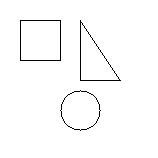
\includegraphics[width=70mm]{zukei-out.png}
    \end{center}
    \caption{zukei-out.pbn}
    \label{fig:zuou}
  \end{minipage}
  \begin{minipage}{0.5\hsize}
    \begin{center}
      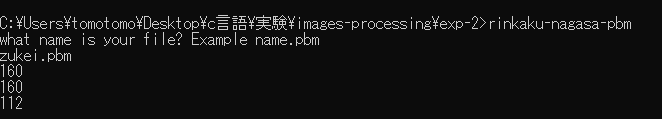
\includegraphics[width=70mm]{zukei-length.png}
    \end{center}
    \caption{出力された長さ}
    \label{fig:zule}
  \end{minipage}
\end{figure}
\lstinputlisting[caption=rinkaku-nagasa-pbm.c]{rinkaku-nagasa-pbm.c}

\end{document}
